\section{PLL: Phase Locked-Loop}

\subsection{Introducci\'on}

Un Phase Locked-Loop, mejor conocido como PLL, es un sistema de control cuya se\~nal de salida tiene la misma frecuencia que la se\~nal de entrada y sigue sus variaciones en frecuencia dentro de un rango acotado. El PLL es muy usado en sistemas de comunicaciones, ya que sus principales aplicaciones son de demodulador de FM o PM y como seguidor o sincronizador de se\~nales que temporalmente var\'ian su frecuencia. A continuaci\'on se analizar\'an ciertos comportamientos del PLL y su aplicaci\'on como demodulador de FM y como multiplicador de frecuencia.

\subsection{Diagrama en bloques del PLL}

El PLL est\'a formado por tres bloques fundamentales para su funcionamiento: un comparador de fase, un filtro pasabajos y un oscilador controlado por tensi\'on (mejor conocido como VCO y que ser\'a estudiado en profundidad en la \'ultima secci\'on). Esta distribuci\'on en bloques es mostrada en la figura \ref{pll}.

\begin{figure}[H] %!ht
	\centering
	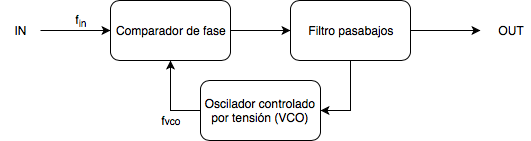
\includegraphics[width=12cm,height=12cm,keepaspectratio]{../EJ2/imagenes/PLL.png}
	\caption{Diagrama en bloques del PLL.}
	\label{pll}
\end{figure}

	\subsubsection{Comparador de fase}
	Del comparador de fase sale una tensi\'on proporcional a la diferencia de fase entre la se\~nal de entrada y aquella que proviene del VCO. Llamando a la tensi\'on de salida del comparador $V_1$, a la ganancia del valor de fase $K_{\phi}$ (la expresi\'on que la determina depende de la forma de implementar el comparador)y a la diferencia de fase entre la se\~nal de entrada y la proveniente del VCO $\Delta_{phi}$:
	
	\begin{equation}
		\begin{cases}
			V_1 = K_{\phi} \cdot \Delta_{\phi} \\
			\Delta_{\phi} = \phi_{in} - \phi_{vco} = \frac{\Delta t}{T}\cdot 2 \pi 	
		\end{cases}
	\end{equation}
	
	\subsubsection{Filtro pasabajos}
	Este filtro se emplea para que el lazo sea estable. Tambi\'en permite un proceso de captura de frecuencias m\'as rapido, un rango de captura mayor y la respuesta del circuito no es sobre amortiguada. Adem\'as, en caso de que se pierda el enganche por interferencias durante el transitorio, el filtro otorga una memoria en el lazo. Por otro lado, la presencia del filtro brinda una ventaja en la demodulaci\'on. La señal que sale del comparador de fase ingresar\'a luego al VCO. Si esta señal tiene un riple, al demodularla puede producir picos no correspondientes a la señal que inicialmente fue modulada.
		
	\subsubsection{VCO: Voltage Controlled Oscillator}
	El VCO es un integrador que genera una frecuencia proporcional a la señal de entrada.
	
\subsection{Respuesta en frecuencia}

\subsection{Respuesta al escal\'on}

	\subsubsection{Factor de calidad a partir del overshoot}

	\subsubsection{Tiempo de establecimiento}

\subsection{Rango de captura y de enganche}

	\subsubsection{Rango de captura}

	\subsubsection{Ranto de enganche}

\subsection{Respuesta transitoria ante distintos filtros}

	\subsubsection{F(s) = 1}
		
	\subsubsection{Filtro pasa bajos}
	
	$F(s) = \frac{1}{\frac{s}{\omega_p} + 1}$
	
	\subsubsection{Filtro con un polo y un cero}
	$F(s) = \frac{\frac{s}{\omega_z} + 1}{\frac{s}{\omega_p} + 1}$

\subsection{Implementaciones con PLL}

	\subsubsection{Demodulador FM }
	
	\subsubsection{Multiplicador de frecuencia}

\subsection{Conclusiones}